\documentclass[12pt,a4paper]{ctexart}
\usepackage[utf8]{inputenc}
\usepackage{amsmath}
\usepackage{amsfonts}
\usepackage{amssymb}
\usepackage{graphicx}
\usepackage{bm}
\usepackage{booktabs}
%\usepackage{draftwatermark}
\usepackage[backend=biber,backref=true%nature,% citestyle=gb7714−2015,backref=true%
]{biblatex}
%参考文献数据源加载 
\addbibresource[location=local]{ref.bib}
\usepackage[table,xcdraw]{xcolor}
\usepackage{float}
%\usepackage[left=3.0cm, right=3.0cm, top=3.5cm, bottom=2.70cm]{geometry}
\title{基于深度学习方法的\\
	自然场景文字识别技术: CRNN+CTC}
\author{Yuan}
\date{\small\today}
\begin{document}

\maketitle
\begin{abstract}
https://zhuanlan.zhihu.com/p/38655369
https://blog.csdn.net/awangpanfeng/article/details/50896303
https://blog.csdn.net/peaceinmind/article/details/51387367
\end{abstract}	
\section{引言}
文字识别,亦称光学字符识别(OCR: Optical Character Recognition)传统上指对输入扫描文档图像进行分析处理,识别出图像中文字信息。场景文字识别(Scene Text Recognition,STR)指识别自然场景图片中的文字信息。

\section{问题描述}
自然场景图像中的文字识别,其难度远大于扫描文档图像中的文字识别,因为它的文字展现形式极其丰富:

\begin{itemize}
	\item 允许多种语言文本混合,字符可以有不同的大小、字体、颜色、亮度、对比度等;
	\item 文本行可能有横向、竖向、弯曲、旋转、扭曲等式样;
	\item 图像中的文字区域还可能会产生变形(透视、仿射变换)、残缺、模糊等现象;
	\item 自然场景图像的背景极其多样。如文字可以出现在平面、曲面或折皱面上;文字区域附近有复杂的干扰纹理、或者非文字区域有近似文字的纹理,比如沙地、草丛、栅栏、砖墙等。
\end{itemize}
\section{CRNN+CTC模型}
使用深度学习方法解决自然场景文字识别的模型非常多,其中有基于注意力机制的模型FAN网络(Focusing Attention Network)\cite{FAN}以及应用注意力机制的2D非规整文字网络\cite{2D-ATTN}。其中CRNN(Convolutional Recurrent Neural Network)\cite{CRNN}是目前较为流行的模型,可识别较长的文本序列,为CRNN+CTC的网络结构,模型包含CNN特征提取层和BLSTM(Bi-direct Long Short Term Memory)\cite{BLSTM}序列特征提取层,能够进行端到端的联合训练。图\ref{fig:blstm}为BLSTM的具体结构。模型的感受野如图\ref{fig:receptive_field}所示,一个字符可能被多个BLSTM单元所覆盖,故需要引入CTC转译。 模型利用BLSTM和CTC\cite{Graves:2006:CTC:1143844.1143891}部件学习字符图像中的上下文关系, 从而有效提升文本识别准确率,使得模型更加鲁棒。预测过程中,前端使用标准的CNN网络提取文本图像的特征,利用BLSTM将特征向量进行融合以提取字符序列的上下文特征,然后得到每列特征的概率分布,最后通过CTC转译进行预测得到文本序列。
\begin{figure}
	\centering
	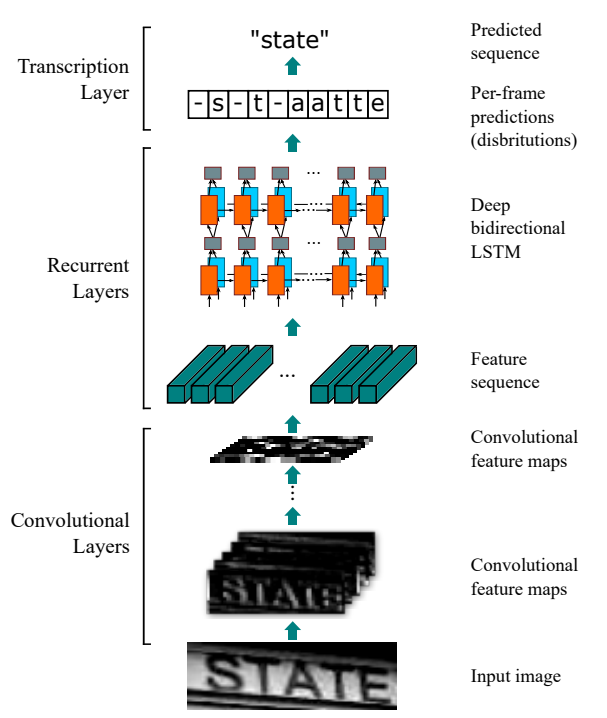
\includegraphics[width=0.7\linewidth]{images/crnn_ctc}
	\caption{CRNN+CTC模型构架}
	\label{fig:crnn_ctc}
\end{figure}

\begin{figure}
	\centering
	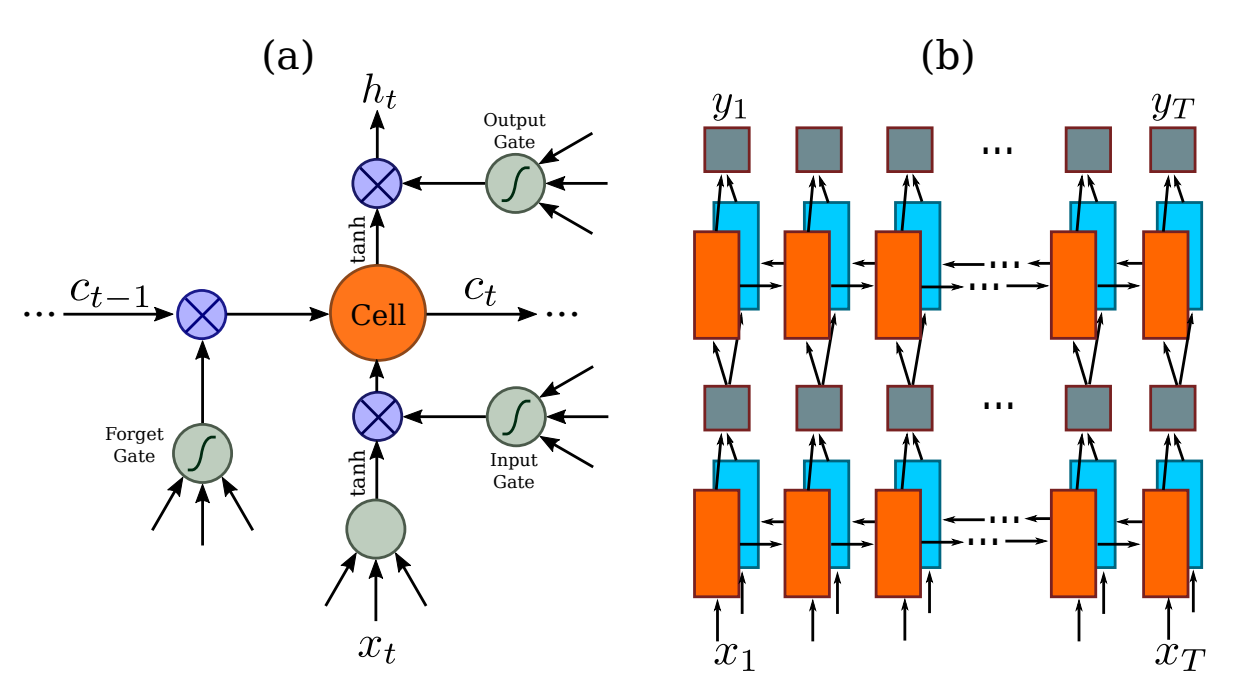
\includegraphics[width=0.7\linewidth]{images/blstm}
	\caption{BLSTM}
	\label{fig:blstm}
\end{figure}
\begin{figure}
	\centering
	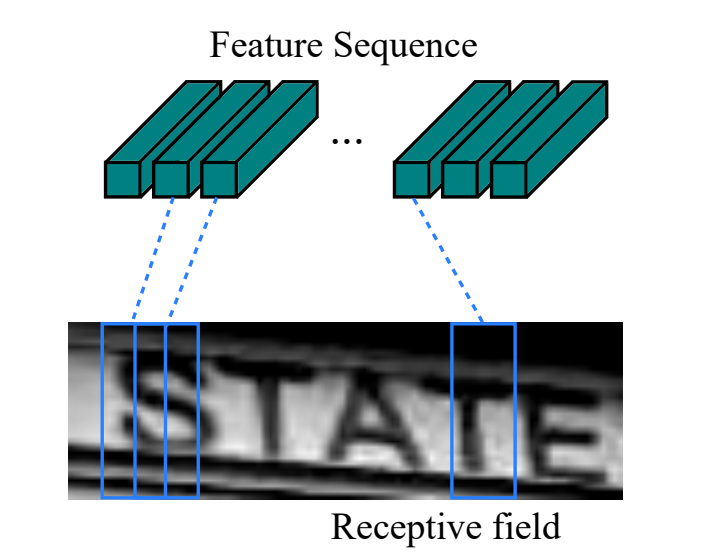
\includegraphics[width=0.5\linewidth]{images/receptive_field}
	\caption{模型感受野}
	\label{fig:receptive_field}
\end{figure}


\section{训练数据集}
目前主流的针对中文汉字的自然场文字识别的数据集主要有Chinese Text in the Wild(CTW)\cite{CTW}及Reading Chinese Text in the Wild(RCTW-17)\cite{RCTW-17}。
\subsection{Chinese Text in the Wild(CTW)}
该数据集包含32285张图像,1018402个中文字符(来自于腾讯街景), 包含平面文本,凸起文本,城市文本,农村文本,低亮度文本,远处文本,部分遮挡文本。图像大小2048*2048,数据集大小为31GB。以(8:1:1)的比例将数据集分为训练集(25887张图像,812872个汉字),测试集(3269张图像,103519个汉字),验证集(3129张图像,103519个汉字)。图\ref{fig:ctw-example}为CTW数据的样张及标注示例。
数据集下载地址:\url{https://ctwdataset.github.io/}
\begin{figure}[H]
	\centering
	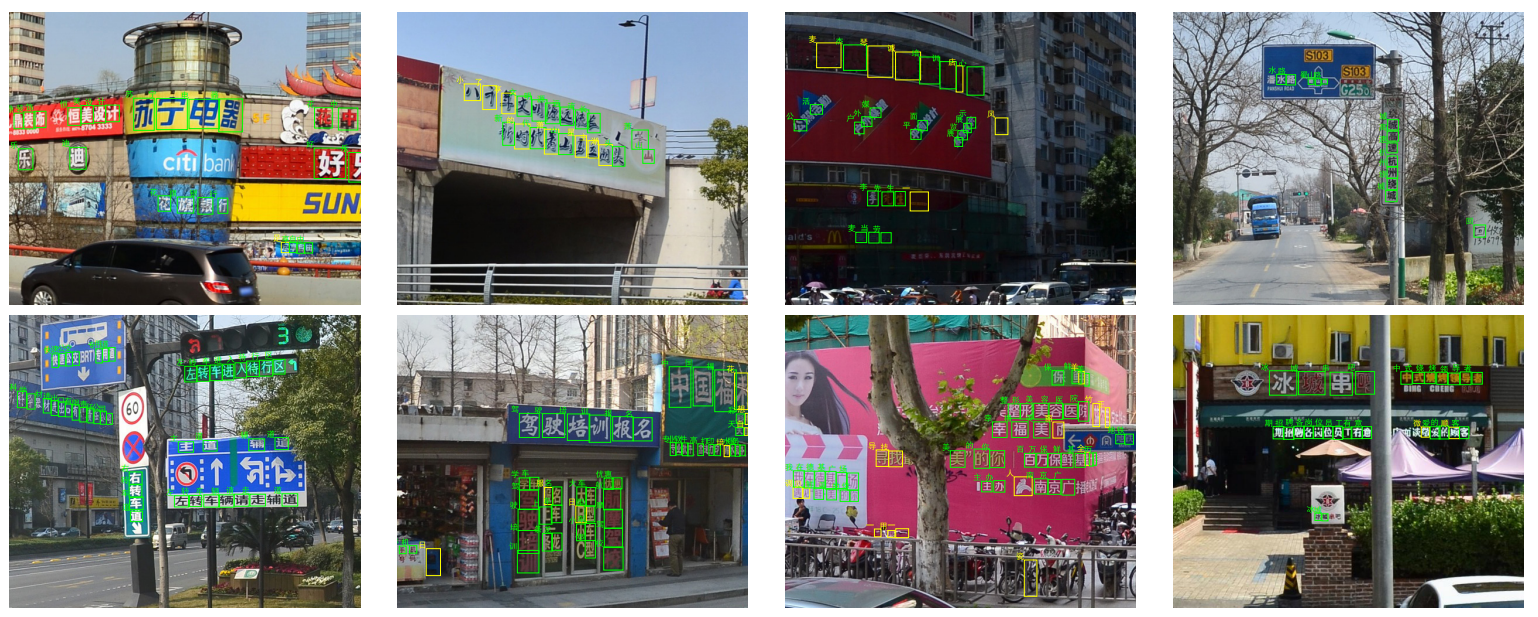
\includegraphics[width=1\linewidth]{images/ctw_example}
	\caption{Chinese Text in the Wild(CTW)数据集样例}
	\label{fig:ctw-example}
\end{figure}
\subsection{Reading Chinese Text in the Wild(RCTW-17)}
该数据集包含12263张图像,训练集8034张,测试集4229张,共11.4GB。大部分图像由手机相机拍摄,含有少量的屏幕截图,图像中包含中文文本与少量英文文本。图像分辨率大小不等。图\ref{fig:rctw17_example}为RCTW-17数据的样张及标注示例。数据集下载地址:\url{http://mclab.eic.hust.edu.cn/icdar2017chinese/dataset.html}
\begin{figure}[H]
	\centering
	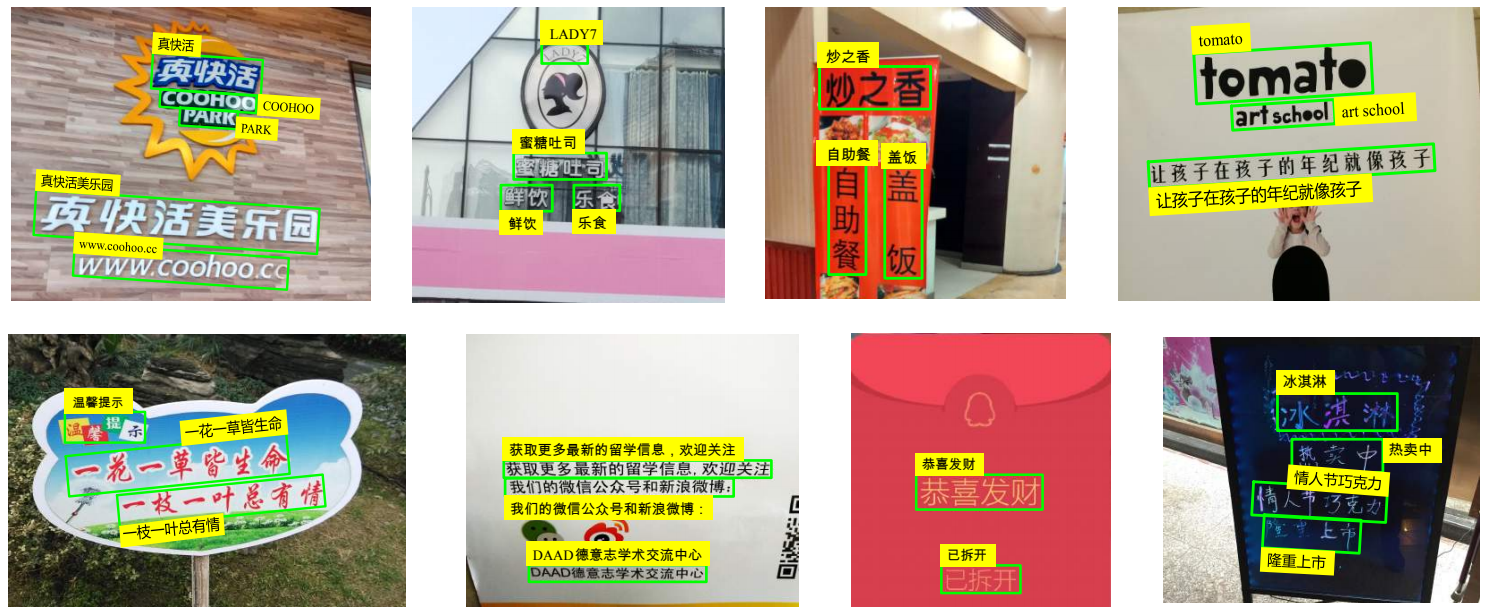
\includegraphics[width=1\linewidth]{images/rctw17_example}
	\caption{Reading Chinese Text in the Wild(RCTW-17)数据集样例}
	\label{fig:rctw17_example}
\end{figure}

\section{总结及展望}
本文使用了HMM建模了拼音序列转汉字序列的标注问题,给出了具体的实验方案并开展了实验,在序列长度小于10的情况下得到近30\%错误率的性能,具有较高的实用价值。值得注意的是模型还有很大的改进空间,例如HMM的状态序列可以用二阶马尔科夫链描述,相对于只考虑前后关系的一阶马尔科夫链会有更好的表现。


\printbibliography[heading=bibliography,title=参考文献]
\end{document}